% Options for packages loaded elsewhere
\PassOptionsToPackage{unicode}{hyperref}
\PassOptionsToPackage{hyphens}{url}
%
\documentclass[
]{article}
\usepackage{amsmath,amssymb}
\usepackage{iftex}
\ifPDFTeX
  \usepackage[T1]{fontenc}
  \usepackage[utf8]{inputenc}
  \usepackage{textcomp} % provide euro and other symbols
\else % if luatex or xetex
  \usepackage{unicode-math} % this also loads fontspec
  \defaultfontfeatures{Scale=MatchLowercase}
  \defaultfontfeatures[\rmfamily]{Ligatures=TeX,Scale=1}
\fi
\usepackage{lmodern}
\ifPDFTeX\else
  % xetex/luatex font selection
\fi
% Use upquote if available, for straight quotes in verbatim environments
\IfFileExists{upquote.sty}{\usepackage{upquote}}{}
\IfFileExists{microtype.sty}{% use microtype if available
  \usepackage[]{microtype}
  \UseMicrotypeSet[protrusion]{basicmath} % disable protrusion for tt fonts
}{}
\makeatletter
\@ifundefined{KOMAClassName}{% if non-KOMA class
  \IfFileExists{parskip.sty}{%
    \usepackage{parskip}
  }{% else
    \setlength{\parindent}{0pt}
    \setlength{\parskip}{6pt plus 2pt minus 1pt}}
}{% if KOMA class
  \KOMAoptions{parskip=half}}
\makeatother
\usepackage{xcolor}
\usepackage[margin=1in]{geometry}
\usepackage{longtable,booktabs,array}
\usepackage{calc} % for calculating minipage widths
% Correct order of tables after \paragraph or \subparagraph
\usepackage{etoolbox}
\makeatletter
\patchcmd\longtable{\par}{\if@noskipsec\mbox{}\fi\par}{}{}
\makeatother
% Allow footnotes in longtable head/foot
\IfFileExists{footnotehyper.sty}{\usepackage{footnotehyper}}{\usepackage{footnote}}
\makesavenoteenv{longtable}
\usepackage{graphicx}
\makeatletter
\def\maxwidth{\ifdim\Gin@nat@width>\linewidth\linewidth\else\Gin@nat@width\fi}
\def\maxheight{\ifdim\Gin@nat@height>\textheight\textheight\else\Gin@nat@height\fi}
\makeatother
% Scale images if necessary, so that they will not overflow the page
% margins by default, and it is still possible to overwrite the defaults
% using explicit options in \includegraphics[width, height, ...]{}
\setkeys{Gin}{width=\maxwidth,height=\maxheight,keepaspectratio}
% Set default figure placement to htbp
\makeatletter
\def\fps@figure{htbp}
\makeatother
\setlength{\emergencystretch}{3em} % prevent overfull lines
\providecommand{\tightlist}{%
  \setlength{\itemsep}{0pt}\setlength{\parskip}{0pt}}
\setcounter{secnumdepth}{-\maxdimen} % remove section numbering
\usepackage[utf8]{inputenc}

\usepackage{setspace}
\doublespacing

\usepackage[version = 4]{mhchem}

% TABLES
\usepackage{tabularx}
\usepackage{multirow}
\usepackage{threeparttable}
\usepackage{booktabs}
\usepackage{rotating}
\usepackage{csvsimple}

% SIUNITX
\usepackage{siunitx}

\sisetup{separate-uncertainty, multi-part-units = repeat}

\newcommand\SIci[4]{\SI{#1}{#2} ({95\%}CI: \SIrange{#3}{#4}{#2})} % Confidence interval
\newcommand\SIcv[1]{\SI{#1}{\percent}} % Coefficient of variation

\DeclareSIUnit[number-unit-product = {}]\degC{\degreeCelsius}
\DeclareSIUnit[number-unit-product = {}]\p{\percent}
\DeclareSIUnit[number-unit-product = \;]\s{\second}
\DeclareSIUnit[number-unit-product = \;]\min{\minute}
\DeclareSIUnit[number-unit-product = \;]\h{\hour}
\DeclareSIUnit[number-unit-product = \;]\d{\day}
\DeclareSIUnit[number-unit-product = \;]\mm{\milli\meter}
\DeclareSIUnit[number-unit-product = \;]\mL{\milli\liter}
\DeclareSIUnit[number-unit-product = \;]\L{\liter}
\DeclareSIUnit[number-unit-product = \;]\cubicm{\cubic\meter}
\DeclareSIUnit[number-unit-product = \;]\kg{\kilo\gram}
\DeclareSIUnit[number-unit-product = \;]\mg{\milli\gram}
\DeclareSIUnit[number-unit-product = \;]\mgL{\milli\gram\per\liter}
\DeclareSIUnit[number-unit-product = \;]\ug{\micro\gram}
\DeclareSIUnit[number-unit-product = \;]\ugL{\micro\gram\per\liter}
\DeclareSIUnit[number-unit-product = \;]\molL{\mole\per\liter}
\DeclareSIUnit[number-unit-product = \;]\mmolL{\milli\mole\per\liter}
\DeclareSIUnit[number-unit-product = \;]\umolL{\micro\mole\per\liter}
\DeclareSIUnit[number-unit-product = \;]\gmol{\gram\per\mole}
\DeclareSIUnit[number-unit-product = \;]\mgkg{\milli\gram\per\kilo\gram}
\DeclareSIUnit[number-unit-product = \;]\gkg{\gram\per\kilo\gram}

% Symbols
\usepackage{amssymb}

% GLOSSARIES
\usepackage{glossaries}

\newacronym{adc}{ADC}{apparent digestibility coefficient}
\newacronym{atp}{ATP}{adenosine triphosphate}
\newacronym{cp}{CP}{crude protein}
\newacronym{cv}{CV}{coefficient of variation}
\newacronym{dm}{DM}{dry matter}
\newacronym{dna}{DNA}{desoxyribonucleic acid}
\newacronym{fao}{FAO}{Food and Agriculture Organization}
\newacronym{fr}{FR}{feeding rate}
\newacronym{imta}{IMTA}{Integrated multitrophic aquaculture}
\newacronym{mle}{MLE}{maximum likelihood estimation}
\newacronym{ras}{RAS}{recirculation aquaculture system}
\newacronym{rna}{RNA}{ribonucleic acid}
\newacronym{usda}{USDA}{United States Department of Agriculture}
\newacronym{usepa}{USEPA}{United States Environmental Protection Agency}
\newacronym{tan}{TAN}{total ammonia nitrogen}
\newacronym{tin}{TIN}{total inorganic nitrogen}
\ifLuaTeX
  \usepackage{selnolig}  % disable illegal ligatures
\fi
\IfFileExists{bookmark.sty}{\usepackage{bookmark}}{\usepackage{hyperref}}
\IfFileExists{xurl.sty}{\usepackage{xurl}}{} % add URL line breaks if available
\urlstyle{same}
\hypersetup{
  pdftitle={Nutrient Contribution},
  pdfauthor={Anıl A. Tellbüscher},
  hidelinks,
  pdfcreator={LaTeX via pandoc}}

\title{Nutrient Contribution}
\usepackage{etoolbox}
\makeatletter
\providecommand{\subtitle}[1]{% add subtitle to \maketitle
  \apptocmd{\@title}{\par {\large #1 \par}}{}{}
}
\makeatother
\subtitle{Assessment of contributions based on estimated assumptions}
\author{Anıl A. Tellbüscher}
\date{Last updated: 13.03.2024}

\begin{document}
\maketitle

{
\setcounter{tocdepth}{2}
\tableofcontents
}
\newpage

\hypertarget{data-import}{%
\section{Data import}\label{data-import}}

\begin{longtable}[]{@{}
  >{\raggedright\arraybackslash}p{(\columnwidth - 2\tabcolsep) * \real{0.5000}}
  >{\raggedright\arraybackslash}p{(\columnwidth - 2\tabcolsep) * \real{0.5000}}@{}}
\toprule\noalign{}
\begin{minipage}[b]{\linewidth}\raggedright
File
\end{minipage} & \begin{minipage}[b]{\linewidth}\raggedright
Content
\end{minipage} \\
\midrule\noalign{}
\endhead
\bottomrule\noalign{}
\endlastfoot
Feed composition APO-SUB-2.xlsx & Composition data of commercial and
experimental fish feeds \\
Water quality APO-SUB-2.xlsx & Composition data of tap and rain water \\
IAFFD FICD.xlsx & Composition of aquafeed raw materials; data downloaded
from www.iaffd.com \\
\end{longtable}

\hypertarget{data-wrangling}{%
\section{Data wrangling}\label{data-wrangling}}

\hypertarget{feed}{%
\subsection{Feed}\label{feed}}

\hypertarget{water}{%
\subsection{Water}\label{water}}

\begin{itemize}
\tightlist
\item
  outliers for rain water were removed
\end{itemize}

\hypertarget{alkalinity-supplements}{%
\subsection{Alkalinity supplements}\label{alkalinity-supplements}}

\newpage

\hypertarget{results}{%
\section{Results}\label{results}}

\hypertarget{feed-1}{%
\subsection{Feed}\label{feed-1}}

\begin{itemize}
\tightlist
\item
  82 commercial feeds
\item
  66 commercial feeds with data from datasheets
\item
  16 commercial feeds with data from literature
\item
  11 experimental feeds
\end{itemize}

\begin{longtable}[]{@{}
  >{\raggedright\arraybackslash}p{(\columnwidth - 16\tabcolsep) * \real{0.2000}}
  >{\raggedright\arraybackslash}p{(\columnwidth - 16\tabcolsep) * \real{0.1538}}
  >{\raggedright\arraybackslash}p{(\columnwidth - 16\tabcolsep) * \real{0.0769}}
  >{\raggedleft\arraybackslash}p{(\columnwidth - 16\tabcolsep) * \real{0.0462}}
  >{\raggedleft\arraybackslash}p{(\columnwidth - 16\tabcolsep) * \real{0.1077}}
  >{\raggedleft\arraybackslash}p{(\columnwidth - 16\tabcolsep) * \real{0.1077}}
  >{\raggedleft\arraybackslash}p{(\columnwidth - 16\tabcolsep) * \real{0.1077}}
  >{\raggedleft\arraybackslash}p{(\columnwidth - 16\tabcolsep) * \real{0.0923}}
  >{\raggedleft\arraybackslash}p{(\columnwidth - 16\tabcolsep) * \real{0.1077}}@{}}
\toprule\noalign{}
\begin{minipage}[b]{\linewidth}\raggedright
category
\end{minipage} & \begin{minipage}[b]{\linewidth}\raggedright
substance
\end{minipage} & \begin{minipage}[b]{\linewidth}\raggedright
unit
\end{minipage} & \begin{minipage}[b]{\linewidth}\raggedleft
n
\end{minipage} & \begin{minipage}[b]{\linewidth}\raggedleft
min
\end{minipage} & \begin{minipage}[b]{\linewidth}\raggedleft
mean
\end{minipage} & \begin{minipage}[b]{\linewidth}\raggedleft
sd
\end{minipage} & \begin{minipage}[b]{\linewidth}\raggedleft
cv
\end{minipage} & \begin{minipage}[b]{\linewidth}\raggedleft
max
\end{minipage} \\
\midrule\noalign{}
\endhead
\bottomrule\noalign{}
\endlastfoot
aquaponic & Ca & gkg & 1 & 15.000 & 15.000 & & & 15.000 \\
aquaponic & K & gkg & 1 & 20.000 & 20.000 & & & 20.000 \\
aquaponic & N & gkg & 3 & 51.200 & 61.333 & 10.410 & 0.170 & 72.000 \\
aquaponic & P & gkg & 3 & 8.000 & 21.667 & 16.503 & 0.762 & 40.000 \\
commercial & Ca & gkg & 5 & 11.700 & 17.560 & 3.686 & 0.210 & 20.000 \\
commercial & Cu & gkg & 4 & 0.005 & 0.020 & 0.019 & 0.933 & 0.046 \\
commercial & Fe & gkg & 4 & 0.040 & 0.209 & 0.237 & 1.136 & 0.544 \\
commercial & K & gkg & 2 & 9.600 & 11.200 & 2.263 & 0.202 & 12.800 \\
commercial & Mg & gkg & 3 & 1.400 & 2.233 & 0.802 & 0.359 & 3.000 \\
commercial & N & gkg & 74 & 40.000 & 63.862 & 11.796 & 0.185 & 89.600 \\
commercial & P & gkg & 68 & 7.000 & 11.662 & 2.444 & 0.210 & 18.000 \\
commercial & S & gkg & 1 & 1.024 & 1.024 & & & 1.024 \\
commercial & Zn & gkg & 4 & 0.090 & 0.207 & 0.127 & 0.613 & 0.384 \\
experimental & Ca & gkg & 11 & 2.760 & 14.646 & 8.410 & 0.574 &
26.710 \\
experimental & Cu & gkg & 8 & 0.013 & 0.016 & 0.003 & 0.179 & 0.021 \\
experimental & Fe & gkg & 8 & 0.121 & 0.348 & 0.297 & 0.854 & 0.850 \\
experimental & K & gkg & 11 & 5.000 & 8.633 & 2.762 & 0.320 & 12.630 \\
experimental & Mg & gkg & 11 & 1.292 & 2.021 & 0.727 & 0.359 & 3.480 \\
experimental & N & gkg & 11 & 59.257 & 64.983 & 4.030 & 0.062 &
70.400 \\
experimental & P & gkg & 11 & 7.172 & 14.104 & 4.940 & 0.350 & 20.700 \\
experimental & S & gkg & 11 & 2.751 & 4.032 & 0.868 & 0.215 & 5.500 \\
experimental & Zn & gkg & 8 & 0.050 & 0.093 & 0.036 & 0.385 & 0.151 \\
old & Ca & gkg & 9 & 11.429 & 22.676 & 8.952 & 0.395 & 36.429 \\
old & Cu & gkg & 9 & 0.006 & 0.021 & 0.015 & 0.728 & 0.046 \\
old & Fe & gkg & 9 & 0.080 & 0.207 & 0.134 & 0.644 & 0.500 \\
old & K & gkg & 9 & 6.571 & 9.485 & 1.979 & 0.209 & 12.286 \\
old & Mg & gkg & 9 & 1.736 & 2.118 & 0.300 & 0.142 & 2.740 \\
old & P & gkg & 9 & 9.286 & 16.252 & 6.371 & 0.392 & 28.143 \\
old & Zn & gkg & 9 & 0.055 & 0.113 & 0.067 & 0.597 & 0.270 \\
\end{longtable}

\hypertarget{statistics}{%
\subsubsection{Statistics}\label{statistics}}

\begin{itemize}
\item
  reliable comparison of nutrient inclusion is only possible for P,
  considering the number of observations in the dataset.
\item
  comparison of commercial data with aquaponics or experimental feed is
  also not meaningful due to low sample size
\item
  P: Aquaponics feeds are richer in P compared with commercial feeds and
  also compared with experimental diets (Tukey test: p \textless{}
  0.05). The smallest difference was found between aquaponics and old
  diets. The difference between them is non-significant.
\end{itemize}

\hypertarget{feed-composition}{%
\subsubsection{Feed composition}\label{feed-composition}}

\includegraphics[width=27.08in]{../output/plots/feed}

\hypertarget{feedstuff-composition}{%
\subsubsection{Feedstuff composition}\label{feedstuff-composition}}

\begin{longtable}[]{@{}llrrrr@{}}
\toprule\noalign{}
cat2 & analyte & n & mean & sd & cv \\
\midrule\noalign{}
\endhead
\bottomrule\noalign{}
\endlastfoot
aquatic & N (g/kg) & 86 & 556.81 & 154.06 & 0.277 \\
aquatic & Fe (mg/kg) & 82 & 258.11 & 132.10 & 0.512 \\
aquatic & Mn (mg/kg) & 84 & 17.26 & 9.02 & 0.522 \\
aquatic & P (g/kg) & 56 & 17.88 & 7.38 & 0.413 \\
aquatic & K (g/kg) & 80 & 8.68 & 3.33 & 0.384 \\
aquatic & Zn (mg/kg) & 84 & 90.88 & 45.03 & 0.495 \\
insect & N (g/kg) & 13 & 544.69 & 120.30 & 0.221 \\
insect & Fe (mg/kg) & 13 & 172.55 & 86.60 & 0.502 \\
insect & Mn (mg/kg) & 4 & 32.12 & 23.23 & 0.723 \\
insect & P (g/kg) & 13 & 10.62 & 4.49 & 0.423 \\
insect & K (g/kg) & 13 & 6.54 & 4.56 & 0.697 \\
insect & Zn (mg/kg) & 13 & 83.28 & 42.72 & 0.513 \\
microbial & N (g/kg) & 19 & 493.26 & 144.74 & 0.293 \\
microbial & Fe (mg/kg) & 17 & 141.40 & 85.45 & 0.604 \\
microbial & Mn (mg/kg) & 16 & 30.05 & 23.30 & 0.775 \\
microbial & P (g/kg) & 18 & 14.02 & 6.55 & 0.468 \\
microbial & K (g/kg) & 15 & 3.83 & 4.26 & 1.110 \\
microbial & Zn (mg/kg) & 16 & 72.12 & 47.80 & 0.663 \\
plant & N (g/kg) & 192 & 340.35 & 228.27 & 0.671 \\
plant & Fe (mg/kg) & 191 & 148.49 & 107.09 & 0.721 \\
plant & Mn (mg/kg) & 171 & 28.28 & 19.09 & 0.675 \\
plant & P (g/kg) & 194 & 6.21 & 3.05 & 0.491 \\
plant & K (g/kg) & 187 & 1.24 & 2.04 & 1.653 \\
plant & Zn (mg/kg) & 191 & 45.51 & 24.86 & 0.546 \\
terrestrial & N (g/kg) & 40 & 649.20 & 171.53 & 0.264 \\
terrestrial & Fe (mg/kg) & 33 & 293.81 & 149.65 & 0.509 \\
terrestrial & Mn (mg/kg) & 40 & 13.21 & 9.69 & 0.733 \\
terrestrial & P (g/kg) & 27 & 14.31 & 9.95 & 0.695 \\
terrestrial & K (g/kg) & 38 & 5.53 & 3.45 & 0.623 \\
terrestrial & Zn (mg/kg) & 40 & 76.15 & 31.29 & 0.411 \\
\end{longtable}

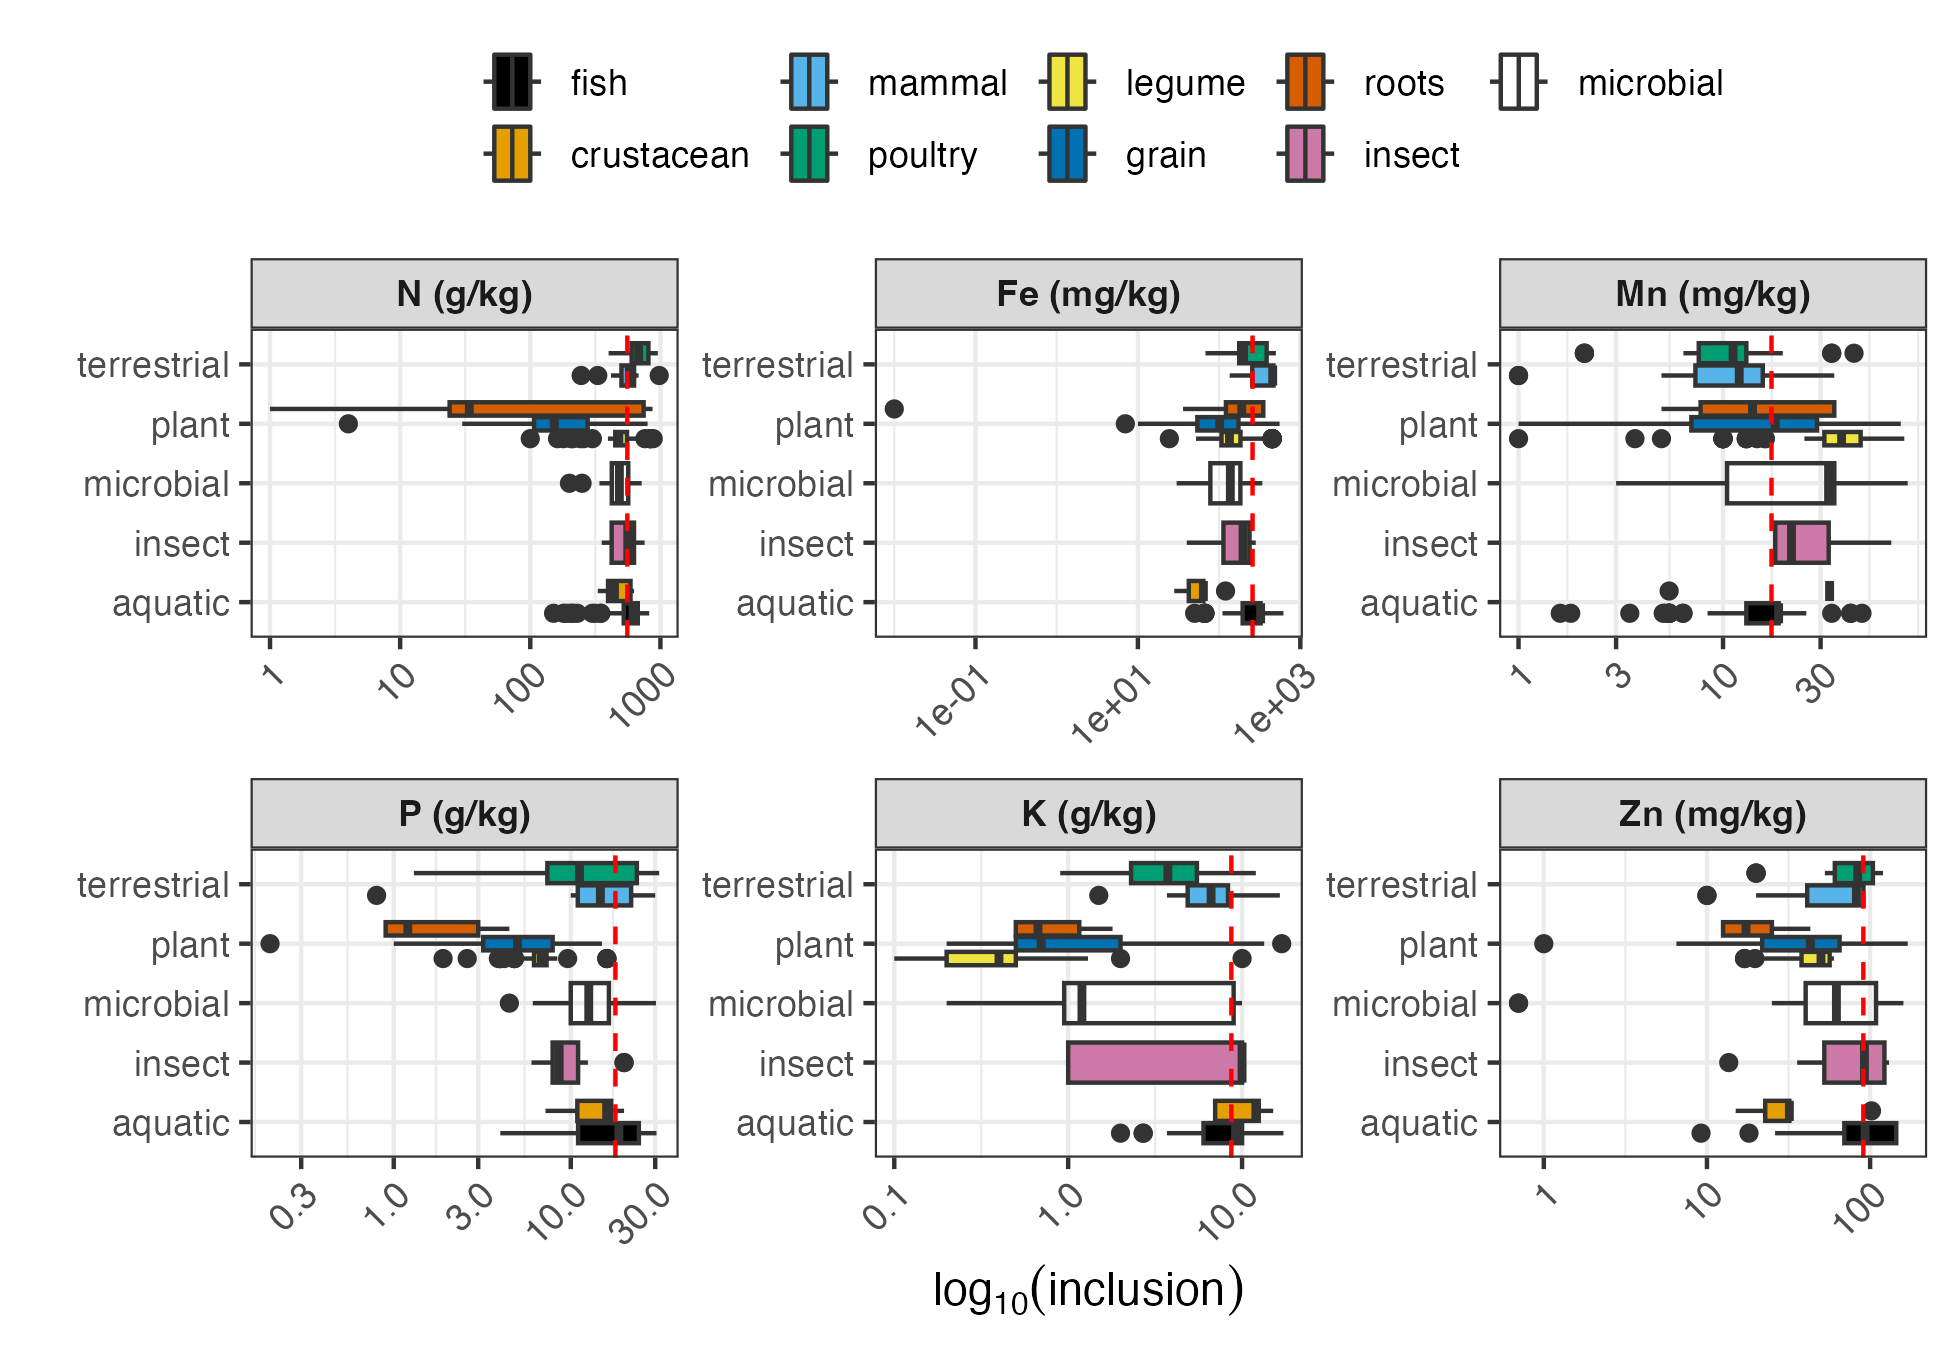
\includegraphics[width=27.08in]{../output/plots/feedstuff_composition}

\hypertarget{water-1}{%
\subsection{Water}\label{water-1}}

\hypertarget{data-origin}{%
\subsubsection{Data origin}\label{data-origin}}

\begin{figure}
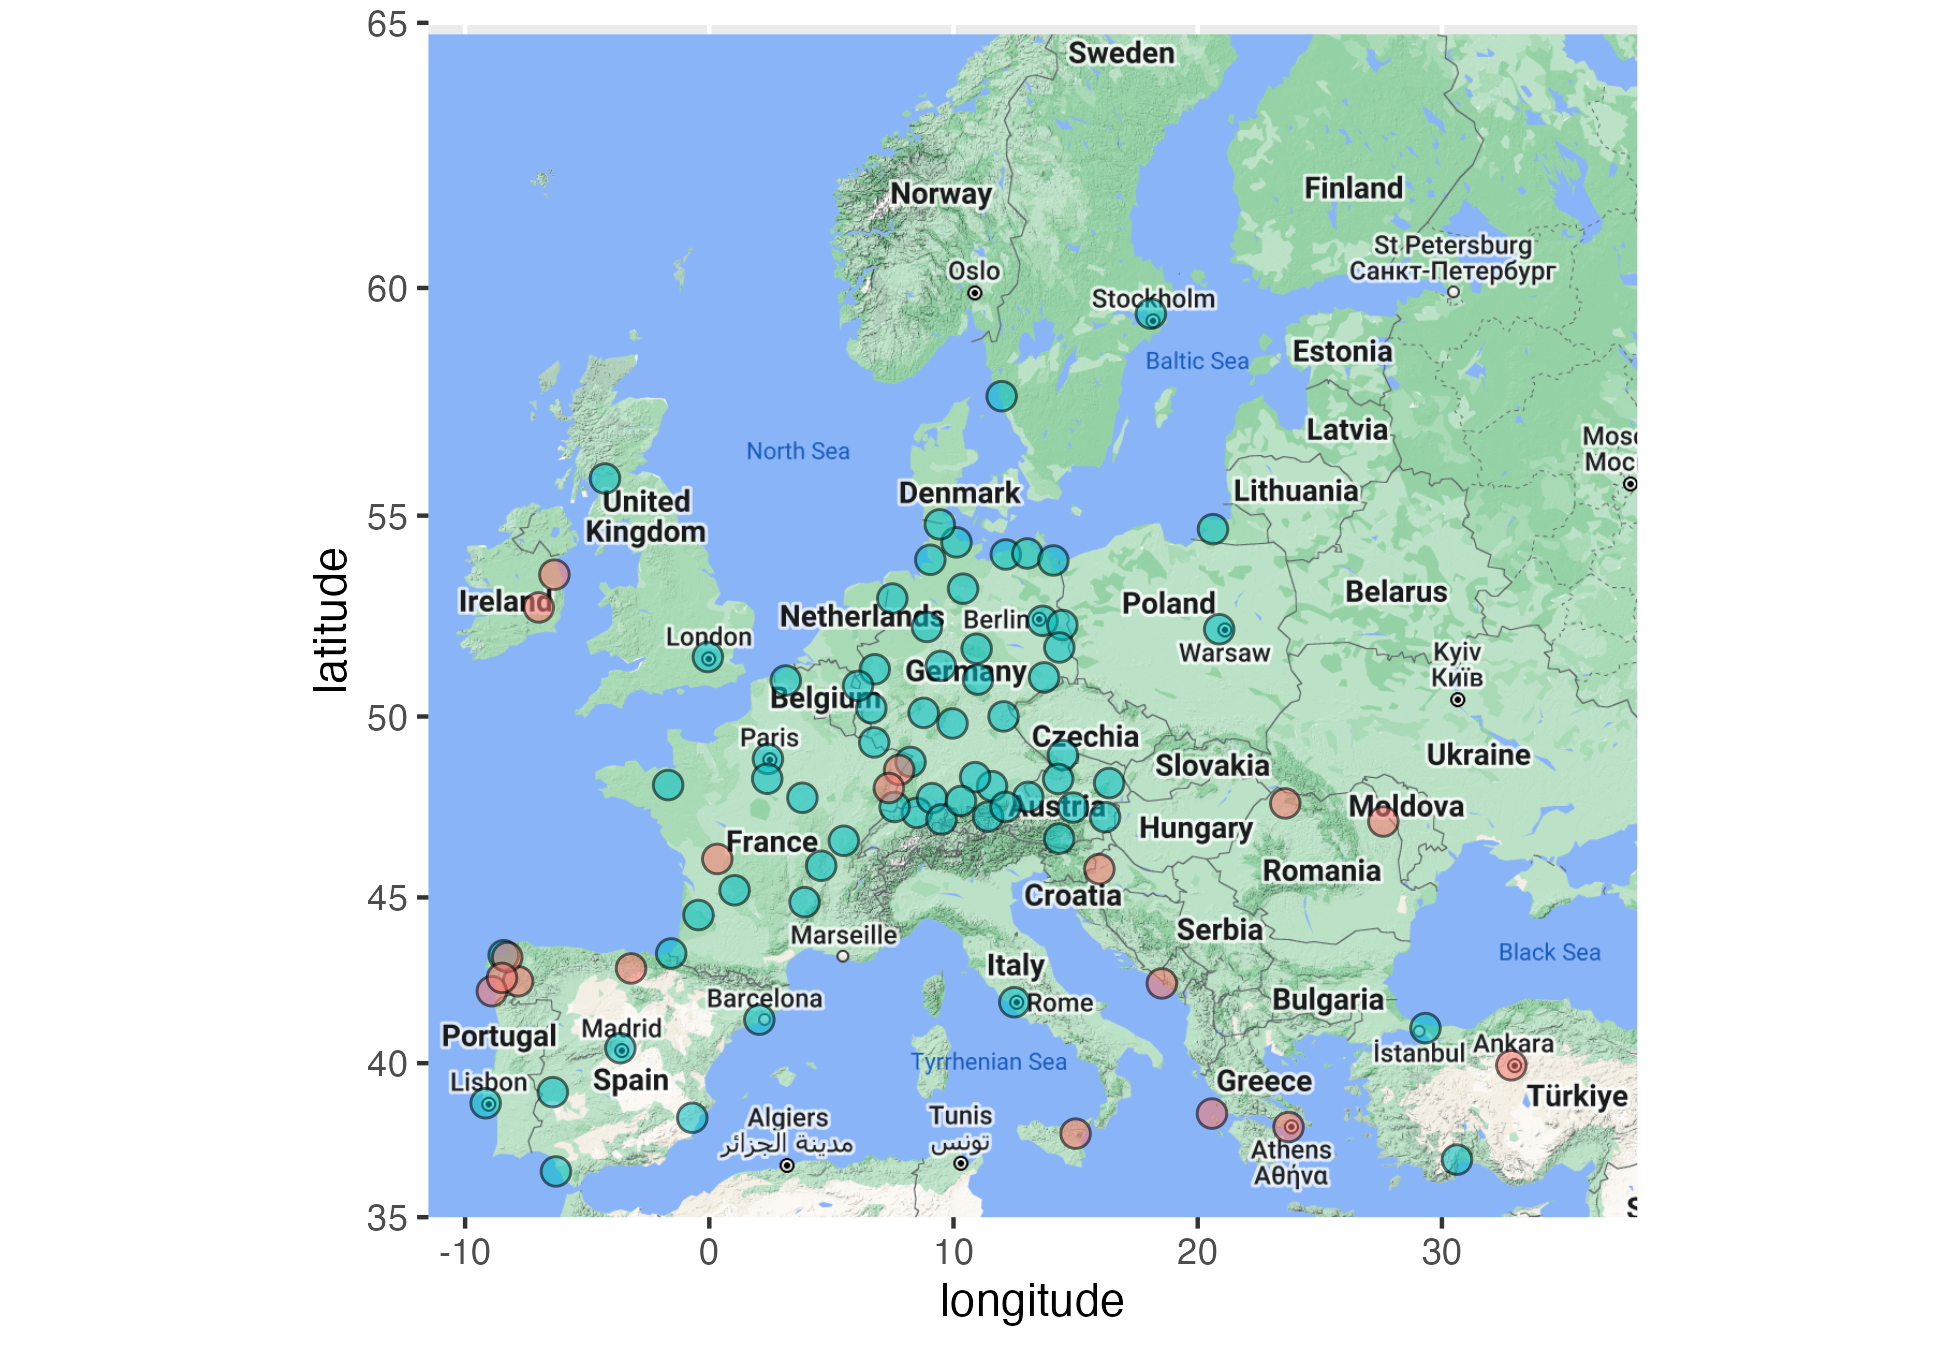
\includegraphics[width=27.08in]{../output/plots/map} \caption{Origins of data included into the water dataset. Blue dots: Drinking water analysis reports. Red dots: Rain water analyses.}\label{fig:unnamed-chunk-16}
\end{figure}

\hypertarget{tap-water}{%
\subsubsection{Tap water}\label{tap-water}}

\begin{itemize}
\tightlist
\item
  71 tap water analysis reports
\end{itemize}

\begin{longtable}[]{@{}llrrrrrr@{}}
\caption{Summary statistics of the chemical composition of tap water.
Data was compiled from analysis reports of water supply companies (n =
71). Mean values were estimated using accepted methods for censored data
(Helsel, 2012). N is the sum of all nitrogenous species.}\tabularnewline
\toprule\noalign{}
analyte & unit & n & min & mean & sd & cv & max \\
\midrule\noalign{}
\endfirsthead
\toprule\noalign{}
analyte & unit & n & min & mean & sd & cv & max \\
\midrule\noalign{}
\endhead
\bottomrule\noalign{}
\endlastfoot
N & µmolL & 62 & 2110.073 & 2110.077 & 0.000 & 0.000 & 2110.073 \\
P & µmolL & 24 & 0.001 & 0.888 & 1.942 & 2.188 & 6.949 \\
K & µmolL & 51 & 2.558 & 65.930 & 66.357 & 1.006 & 358.072 \\
Ca & µmolL & 57 & 82.339 & 1484.005 & 815.786 & 0.550 & 3418.334 \\
Mg & µmolL & 57 & 37.029 & 462.482 & 333.265 & 0.721 & 1781.526 \\
S & µmolL & 58 & 6.746 & 137.463 & 139.926 & 1.018 & 630.839 \\
B & µmolL & 40 & 0.462 & 4.988 & 11.570 & 2.319 & 59.014 \\
Fe & µmolL & 62 & 0.000 & 0.581 & 2.975 & 5.117 & 23.637 \\
Mn & µmolL & 54 & 0.004 & 0.064 & 0.126 & 1.958 & 0.735 \\
Cu & µmolL & 45 & 0.002 & 0.232 & 0.930 & 4.017 & 4.721 \\
Zn & µmolL & 13 & 0.008 & 0.235 & 0.926 & 3.946 & 3.059 \\
Ni & µmolL & 40 & 0.003 & 0.033 & 0.051 & 1.534 & 0.235 \\
Mo & µmolL & 7 & 0.005 & 0.008 & 0.016 & 2.092 & 0.052 \\
Na & µmolL & 56 & 4.350 & 839.220 & 910.089 & 1.084 & 4697.742 \\
Cl & µmolL & 50 & 2.821 & 774.340 & 705.306 & 0.911 & 3300.144 \\
Al & µmolL & 50 & 0.041 & 0.651 & 0.919 & 1.410 & 4.485 \\
\end{longtable}

\hypertarget{rain-water}{%
\subsubsection{Rain water}\label{rain-water}}

\begin{itemize}
\tightlist
\item
  18 rain water analyses from literature
\item
  13 studies from which the data was derived
\end{itemize}

\begin{longtable}[]{@{}llrrrrrr@{}}
\caption{Summary statistics of rainwater composition data (n = 18).
Analytes with less than 5 dataset records were removed. Outliers were
identified by calculating the interquartile range (IQR). Values
\textgreater{} 1.5 x IQR were removed from the dataset.}\tabularnewline
\toprule\noalign{}
analyte & unit & n & min & mean & sd & cv & max \\
\midrule\noalign{}
\endfirsthead
\toprule\noalign{}
analyte & unit & n & min & mean & sd & cv & max \\
\midrule\noalign{}
\endhead
\bottomrule\noalign{}
\endlastfoot
Ca & µmolL & 14 & 8.98 & 60.8 & 41.19 & 0.677 & 135.5 \\
Cl & µmolL & 14 & 20.14 & 96.5 & 52.18 & 0.541 & 197.4 \\
K & µmolL & 13 & 9.78 & 27.5 & 21.30 & 0.775 & 82.8 \\
Mg & µmolL & 13 & 4.59 & 12.9 & 5.44 & 0.421 & 24.7 \\
N & µmolL & 16 & 0.00 & 90.7 & 52.47 & 0.579 & 205.3 \\
Na & µmolL & 15 & 15.61 & 94.8 & 70.08 & 0.739 & 261.0 \\
S & µmolL & 16 & 16.17 & 44.6 & 24.22 & 0.543 & 88.5 \\
\end{longtable}

\hypertarget{combined}{%
\subsubsection{Combined}\label{combined}}

\begin{longtable}[]{@{}llrrlr@{}}
\toprule\noalign{}
analyte & unit & mean\_tap & mean\_rain & significance & tap:rain
ratio \\
\midrule\noalign{}
\endhead
\bottomrule\noalign{}
\endlastfoot
N & µmolL & 2110.077 & 90.7 & lower & 23 \\
P & µmolL & 0.888 & & & \\
K & µmolL & 65.930 & 27.5 & lower & 2 \\
Ca & µmolL & 1484.005 & 60.8 & lower & 24 \\
Mg & µmolL & 462.482 & 12.9 & lower & 36 \\
S & µmolL & 137.463 & 44.6 & lower & 3 \\
B & µmolL & 4.988 & & & \\
Fe & µmolL & 0.581 & & & \\
Mn & µmolL & 0.064 & & & \\
Cu & µmolL & 0.232 & & & \\
Zn & µmolL & 0.235 & & & \\
Ni & µmolL & 0.033 & & & \\
Mo & µmolL & 0.008 & & & \\
Na & µmolL & 839.220 & 94.8 & lower & 9 \\
Cl & µmolL & 774.340 & 96.5 & lower & 8 \\
Al & µmolL & 0.651 & & & \\
\end{longtable}

\begin{itemize}
\tightlist
\item
  All substance concentrations that are known for both tap and rain
  water are significantly lower in rain water (p \textless{} 0.05).
\end{itemize}

\hypertarget{alkalinity-supplements-1}{%
\subsection{Alkalinity supplements}\label{alkalinity-supplements-1}}

\newpage

\hypertarget{nutrient-contribution}{%
\section{Nutrient contribution}\label{nutrient-contribution}}

\hypertarget{initial-assumptions}{%
\subsection{Initial assumptions}\label{initial-assumptions}}

We assume a recirculation aquaculture system (RAS) has a total volume of
\si{\cubicm} of which \si{\cubicm} are used as rearing volume for the
stock. Furthermore, we assume a stocking density of \si{\kg\per\cubicm},
referred to the rearing volume of the system. The feeding rate shall be
set to \si{\p\per\d} of the total biomass and a water exchange rate of
\si{\p\per\d} of the total system volume shall be maintained.

Based on these inputs, a biomass of \si{\kg}, a total weight of \si{\kg}
feed fed per day, a daily exchanged volume of \si{\cubicm\per\d}
freshwater and \si{\L\per\kg} exchanged water per weight unit feed fed
is calculated.

To estimate the mass contribution of source water and feed to the total
amount of nutrients that are entering the system, it is assumed that the
RAS operator is using tap water as freshwater source and analysis
results from water treatment plants are thus taken as data input.
Furthermore, the average of the nutrient profile of a number of
commercial fish feeds is used.

\hypertarget{data-preparation}{%
\subsection{Data preparation}\label{data-preparation}}

\hypertarget{feed-2}{%
\subsubsection{Feed}\label{feed-2}}

\hypertarget{consideration-of-digestibility}{%
\paragraph{Consideration of
digestibility}\label{consideration-of-digestibility}}

Assumptions with regards to the digestibility of nutrients in the feeds
are the following:

\begin{itemize}
\tightlist
\item
  \textbf{N} ADC ranging between 85-95\%
\item
  \textbf{P} ADC ranging between 35-45\% {[}@Sugiura2018{]}
\item
  all other nutrient ADC ranging between 45-55\%
\end{itemize}

\hypertarget{consideration-of-retention}{%
\paragraph{Consideration of
retention}\label{consideration-of-retention}}

\textbf{Retention} assumptions are based on {[}@Roy2022{]}. These were
derived from Tilapia, though.

The amount of daily feed fed was normalised to 1 kg of feed instead of
going for the initial assumptions. This makes it better comparable.

\hypertarget{water-2}{%
\subsubsection{Water}\label{water-2}}

\hypertarget{tap-water-1}{%
\paragraph{Tap water}\label{tap-water-1}}

\hypertarget{rain-water-1}{%
\paragraph{Rain water}\label{rain-water-1}}

\hypertarget{empirical-probability-analysis}{%
\subsection{Empirical probability
analysis}\label{empirical-probability-analysis}}

\hypertarget{without-retention}{%
\subsubsection{Without retention}\label{without-retention}}

\hypertarget{retention---tap-water}{%
\subsubsection{Retention - Tap water}\label{retention---tap-water}}

After consideration of nutrient digestibility, two scenarios occur: 1.
still majority of nutrient input by feed 2. 3. equal contribution of
water and feed possible

\begin{itemize}
\tightlist
\item
  tap water can contribute a share of N comparable to aquafeeds in some
  cases
\item
  the probability that the majority of K will originate from aquafeeds
  is 100\%
\item
\end{itemize}

\hypertarget{retention---rain-water}{%
\subsubsection{Retention - Rain water}\label{retention---rain-water}}

\hypertarget{combined-1}{%
\subsubsection{Combined}\label{combined-1}}

\begin{verbatim}
## $x
## [1] "Share of total nutrient input (%)"
## 
## $y
## [1] ""
## 
## attr(,"class")
## [1] "labels"
\end{verbatim}

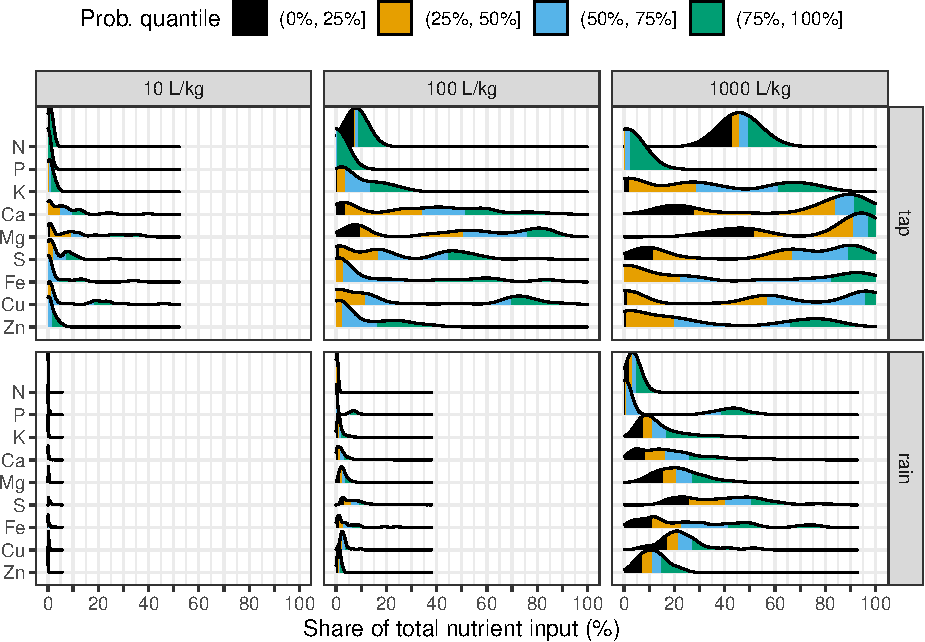
\includegraphics{analysis_files/figure-latex/unnamed-chunk-57-1.pdf}

\hypertarget{variability}{%
\subsubsection{Variability}\label{variability}}

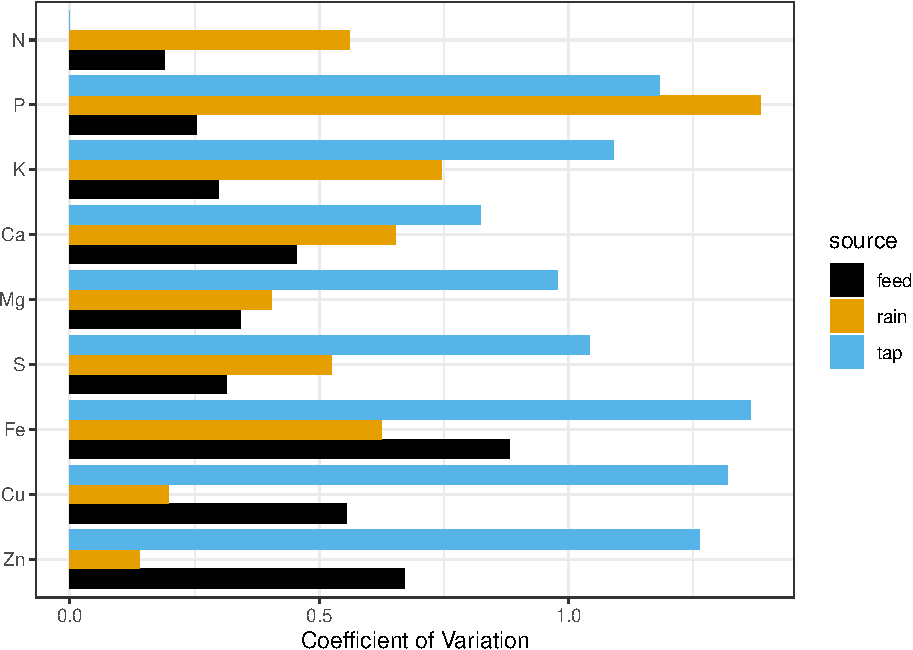
\includegraphics{analysis_files/figure-latex/plot_variability-1.pdf}

It can be seen that tap water is the predominant source of variability
in the results Feed was found to have the lowest variability (\gls{cv}
\textless{} 0.5) of all nutrient sources for the major nutrients
(nitrogen, phosphorus, the earth alkaline metals, potassium, and
sulfur). The variability in the mass fractions of transition metals in
feeds, on the other hand, is significantly higher. However, the
variability is always lower than that found for tap water sources.

The highest variability in the data can be found in tap water with
exception of phosphorus, which is more variable in rain

\begin{longtable}[]{@{}
  >{\raggedright\arraybackslash}p{(\columnwidth - 16\tabcolsep) * \real{0.1316}}
  >{\raggedright\arraybackslash}p{(\columnwidth - 16\tabcolsep) * \real{0.1053}}
  >{\raggedleft\arraybackslash}p{(\columnwidth - 16\tabcolsep) * \real{0.2105}}
  >{\raggedleft\arraybackslash}p{(\columnwidth - 16\tabcolsep) * \real{0.0921}}
  >{\raggedleft\arraybackslash}p{(\columnwidth - 16\tabcolsep) * \real{0.0921}}
  >{\raggedleft\arraybackslash}p{(\columnwidth - 16\tabcolsep) * \real{0.0921}}
  >{\raggedleft\arraybackslash}p{(\columnwidth - 16\tabcolsep) * \real{0.0921}}
  >{\raggedleft\arraybackslash}p{(\columnwidth - 16\tabcolsep) * \real{0.0921}}
  >{\raggedleft\arraybackslash}p{(\columnwidth - 16\tabcolsep) * \real{0.0921}}@{}}
\caption{Quantiles of percentage contribution to the total nutrient
input into an aquaculture system as shown in the figure
before.}\tabularnewline
\toprule\noalign{}
\begin{minipage}[b]{\linewidth}\raggedright
substance
\end{minipage} & \begin{minipage}[b]{\linewidth}\raggedright
source2
\end{minipage} & \begin{minipage}[b]{\linewidth}\raggedleft
dailyFreshwater
\end{minipage} & \begin{minipage}[b]{\linewidth}\raggedleft
median
\end{minipage} & \begin{minipage}[b]{\linewidth}\raggedleft
0-20
\end{minipage} & \begin{minipage}[b]{\linewidth}\raggedleft
20-40
\end{minipage} & \begin{minipage}[b]{\linewidth}\raggedleft
40-60
\end{minipage} & \begin{minipage}[b]{\linewidth}\raggedleft
60-80
\end{minipage} & \begin{minipage}[b]{\linewidth}\raggedleft
80-100
\end{minipage} \\
\midrule\noalign{}
\endfirsthead
\toprule\noalign{}
\begin{minipage}[b]{\linewidth}\raggedright
substance
\end{minipage} & \begin{minipage}[b]{\linewidth}\raggedright
source2
\end{minipage} & \begin{minipage}[b]{\linewidth}\raggedleft
dailyFreshwater
\end{minipage} & \begin{minipage}[b]{\linewidth}\raggedleft
median
\end{minipage} & \begin{minipage}[b]{\linewidth}\raggedleft
0-20
\end{minipage} & \begin{minipage}[b]{\linewidth}\raggedleft
20-40
\end{minipage} & \begin{minipage}[b]{\linewidth}\raggedleft
40-60
\end{minipage} & \begin{minipage}[b]{\linewidth}\raggedleft
60-80
\end{minipage} & \begin{minipage}[b]{\linewidth}\raggedleft
80-100
\end{minipage} \\
\midrule\noalign{}
\endhead
\bottomrule\noalign{}
\endlastfoot
Ca & tap & 10 & 5.007 & 0.332 & 3.595 & 6.424 & 11.830 & 41.577 \\
Ca & tap & 100 & 34.514 & 3.223 & 27.161 & 40.707 & 57.295 & 87.679 \\
Ca & tap & 1000 & 84.052 & 24.981 & 78.853 & 87.286 & 93.064 & 98.614 \\
Ca & rain & 10 & 0.197 & 0.071 & 0.153 & 0.244 & 0.410 & 2.743 \\
Ca & rain & 100 & 1.937 & 0.701 & 1.507 & 2.384 & 3.950 & 22.001 \\
Ca & rain & 1000 & 16.494 & 6.591 & 13.267 & 19.630 & 29.138 & 73.826 \\
Cu & tap & 10 & 1.310 & 0.010 & 1.073 & 1.631 & 19.806 & 48.290 \\
Cu & tap & 100 & 11.722 & 0.099 & 9.789 & 14.226 & 71.179 & 90.327 \\
Cu & tap & 1000 & 57.040 & 0.982 & 52.042 & 62.385 & 96.108 & 98.941 \\
Cu & rain & 10 & 0.275 & 0.198 & 0.255 & 0.303 & 0.386 & 1.148 \\
Cu & rain & 100 & 2.688 & 1.945 & 2.496 & 2.945 & 3.726 & 10.403 \\
Cu & rain & 1000 & 21.641 & 16.552 & 20.383 & 23.279 & 27.903 &
53.727 \\
Fe & tap & 10 & 0.286 & 0.000 & 0.094 & 0.442 & 7.225 & 37.079 \\
Fe & tap & 100 & 2.788 & 0.001 & 0.928 & 4.252 & 43.781 & 85.492 \\
Fe & tap & 1000 & 22.287 & 0.005 & 8.568 & 30.753 & 88.620 & 98.331 \\
Fe & rain & 10 & 0.292 & 0.109 & 0.177 & 0.406 & 0.828 & 3.524 \\
Fe & rain & 100 & 2.844 & 1.077 & 1.744 & 3.920 & 7.709 & 26.754 \\
Fe & rain & 1000 & 22.641 & 9.815 & 15.077 & 28.975 & 45.514 & 78.507 \\
K & tap & 10 & 0.398 & 0.017 & 0.285 & 0.572 & 1.847 & 3.859 \\
K & tap & 100 & 3.844 & 0.168 & 2.775 & 5.444 & 15.837 & 28.645 \\
K & tap & 1000 & 28.557 & 1.659 & 22.207 & 36.537 & 65.299 & 80.057 \\
K & rain & 10 & 0.125 & 0.076 & 0.105 & 0.144 & 0.236 & 0.920 \\
K & rain & 100 & 1.235 & 0.754 & 1.041 & 1.417 & 2.314 & 8.493 \\
K & rain & 1000 & 11.111 & 7.064 & 9.520 & 12.565 & 19.151 & 48.137 \\
Mg & tap & 10 & 9.279 & 0.891 & 6.555 & 12.192 & 26.388 & 39.899 \\
Mg & tap & 100 & 50.562 & 8.251 & 41.228 & 58.131 & 78.189 & 86.909 \\
Mg & tap & 1000 & 91.093 & 47.350 & 87.523 & 93.281 & 97.286 & 98.516 \\
Mg & rain & 10 & 0.264 & 0.163 & 0.231 & 0.299 & 0.404 & 0.912 \\
Mg & rain & 100 & 2.581 & 1.606 & 2.259 & 2.911 & 3.902 & 8.424 \\
Mg & rain & 1000 & 20.947 & 14.035 & 18.773 & 23.070 & 28.881 &
47.914 \\
N & tap & 10 & 0.832 & 0.725 & 0.797 & 0.865 & 0.994 & 1.524 \\
N & tap & 100 & 7.741 & 6.804 & 7.434 & 8.024 & 9.123 & 13.400 \\
N & tap & 1000 & 45.625 & 42.200 & 44.541 & 46.594 & 50.098 & 60.744 \\
N & rain & 10 & 0.036 & 0.015 & 0.032 & 0.041 & 0.054 & 0.150 \\
N & rain & 100 & 0.362 & 0.154 & 0.320 & 0.408 & 0.534 & 1.484 \\
N & rain & 1000 & 3.503 & 1.523 & 3.107 & 3.940 & 5.097 & 13.088 \\
P & tap & 10 & 0.003 & 0.000 & 0.003 & 0.004 & 0.025 & 0.048 \\
P & tap & 100 & 0.034 & 0.000 & 0.027 & 0.040 & 0.249 & 0.478 \\
P & tap & 1000 & 0.341 & 0.001 & 0.272 & 0.403 & 2.438 & 4.584 \\
P & rain & 10 & 0.007 & 0.004 & 0.006 & 0.008 & 0.693 & 1.323 \\
P & rain & 100 & 0.070 & 0.039 & 0.057 & 0.083 & 6.519 & 11.821 \\
P & rain & 1000 & 0.693 & 0.392 & 0.572 & 0.819 & 41.085 & 57.276 \\
S & tap & 10 & 1.972 & 0.110 & 1.655 & 2.687 & 8.038 & 29.263 \\
S & tap & 100 & 16.750 & 1.088 & 14.404 & 21.634 & 46.639 & 80.533 \\
S & tap & 1000 & 66.800 & 9.906 & 62.725 & 73.408 & 89.734 & 97.640 \\
S & rain & 10 & 0.662 & 0.312 & 0.525 & 0.795 & 1.111 & 5.484 \\
S & rain & 100 & 6.252 & 3.032 & 5.011 & 7.417 & 10.104 & 36.716 \\
S & rain & 1000 & 40.007 & 23.817 & 34.533 & 44.478 & 52.919 & 85.298 \\
Zn & tap & 10 & 0.244 & 0.008 & 0.143 & 0.286 & 2.170 & 6.064 \\
Zn & tap & 100 & 2.391 & 0.083 & 1.412 & 2.788 & 18.153 & 39.228 \\
Zn & tap & 1000 & 19.677 & 0.829 & 12.532 & 22.288 & 68.924 & 86.586 \\
Zn & rain & 10 & 0.126 & 0.074 & 0.108 & 0.138 & 0.181 & 0.322 \\
Zn & rain & 100 & 1.243 & 0.738 & 1.065 & 1.361 & 1.782 & 3.127 \\
Zn & rain & 1000 & 11.181 & 6.917 & 9.721 & 12.123 & 15.360 & 24.400 \\
\end{longtable}

\begin{longtable}[]{@{}
  >{\raggedright\arraybackslash}p{(\columnwidth - 16\tabcolsep) * \real{0.1370}}
  >{\raggedright\arraybackslash}p{(\columnwidth - 16\tabcolsep) * \real{0.1096}}
  >{\raggedleft\arraybackslash}p{(\columnwidth - 16\tabcolsep) * \real{0.2192}}
  >{\raggedleft\arraybackslash}p{(\columnwidth - 16\tabcolsep) * \real{0.0959}}
  >{\raggedleft\arraybackslash}p{(\columnwidth - 16\tabcolsep) * \real{0.0822}}
  >{\raggedleft\arraybackslash}p{(\columnwidth - 16\tabcolsep) * \real{0.0822}}
  >{\raggedleft\arraybackslash}p{(\columnwidth - 16\tabcolsep) * \real{0.0822}}
  >{\raggedleft\arraybackslash}p{(\columnwidth - 16\tabcolsep) * \real{0.0959}}
  >{\raggedleft\arraybackslash}p{(\columnwidth - 16\tabcolsep) * \real{0.0959}}@{}}
\caption{Quantiles of percentage contribution to the total nutrient
input into an aquaculture system as shown in the figure
before.}\tabularnewline
\toprule\noalign{}
\begin{minipage}[b]{\linewidth}\raggedright
substance
\end{minipage} & \begin{minipage}[b]{\linewidth}\raggedright
source2
\end{minipage} & \begin{minipage}[b]{\linewidth}\raggedleft
dailyFreshwater
\end{minipage} & \begin{minipage}[b]{\linewidth}\raggedleft
median
\end{minipage} & \begin{minipage}[b]{\linewidth}\raggedleft
0-20
\end{minipage} & \begin{minipage}[b]{\linewidth}\raggedleft
20-40
\end{minipage} & \begin{minipage}[b]{\linewidth}\raggedleft
40-60
\end{minipage} & \begin{minipage}[b]{\linewidth}\raggedleft
60-80
\end{minipage} & \begin{minipage}[b]{\linewidth}\raggedleft
80-100
\end{minipage} \\
\midrule\noalign{}
\endfirsthead
\toprule\noalign{}
\begin{minipage}[b]{\linewidth}\raggedright
substance
\end{minipage} & \begin{minipage}[b]{\linewidth}\raggedright
source2
\end{minipage} & \begin{minipage}[b]{\linewidth}\raggedleft
dailyFreshwater
\end{minipage} & \begin{minipage}[b]{\linewidth}\raggedleft
median
\end{minipage} & \begin{minipage}[b]{\linewidth}\raggedleft
0-20
\end{minipage} & \begin{minipage}[b]{\linewidth}\raggedleft
20-40
\end{minipage} & \begin{minipage}[b]{\linewidth}\raggedleft
40-60
\end{minipage} & \begin{minipage}[b]{\linewidth}\raggedleft
60-80
\end{minipage} & \begin{minipage}[b]{\linewidth}\raggedleft
80-100
\end{minipage} \\
\midrule\noalign{}
\endhead
\bottomrule\noalign{}
\endlastfoot
N & rain & 100 & 0.362 & 0.154 & 0.320 & 0.408 & 0.534 & 1.48 \\
Zn & rain & 100 & 1.243 & 0.738 & 1.065 & 1.361 & 1.782 & 3.13 \\
Mg & rain & 100 & 2.581 & 1.606 & 2.259 & 2.911 & 3.902 & 8.42 \\
K & rain & 100 & 1.235 & 0.754 & 1.041 & 1.417 & 2.314 & 8.49 \\
Cu & rain & 100 & 2.688 & 1.945 & 2.496 & 2.945 & 3.726 & 10.40 \\
P & rain & 100 & 0.070 & 0.039 & 0.057 & 0.083 & 6.519 & 11.82 \\
Ca & rain & 100 & 1.937 & 0.701 & 1.507 & 2.384 & 3.950 & 22.00 \\
Fe & rain & 100 & 2.844 & 1.077 & 1.744 & 3.920 & 7.709 & 26.75 \\
S & rain & 100 & 6.252 & 3.032 & 5.011 & 7.417 & 10.104 & 36.72 \\
\end{longtable}

\hypertarget{alkalinity-supplements-2}{%
\subsection{Alkalinity supplements}\label{alkalinity-supplements-2}}

\begin{longtable}[]{@{}lrrrr@{}}
\caption{Percentage contribution of selected alkalinity supplements to
the nutrient budget at different levels of makeup water supplied to the
system.}\tabularnewline
\toprule\noalign{}
Substance & Makeup water & Alkalinity suppl. & Feed & Water \\
\midrule\noalign{}
\endfirsthead
\toprule\noalign{}
Substance & Makeup water & Alkalinity suppl. & Feed & Water \\
\midrule\noalign{}
\endhead
\bottomrule\noalign{}
\endlastfoot
Ca & 10 & 75.7 & 23.03 & 1.315 \\
K & 10 & 91.6 & 8.30 & 0.068 \\
Mg & 10 & 94.4 & 4.83 & 0.751 \\
Ca & 100 & 67.6 & 20.60 & 11.756 \\
K & 100 & 91.1 & 8.25 & 0.677 \\
Mg & 100 & 88.4 & 4.52 & 7.033 \\
Ca & 1000 & 32.9 & 10.01 & 57.122 \\
K & 1000 & 85.8 & 7.77 & 6.383 \\
Mg & 1000 & 54.2 & 2.77 & 43.071 \\
\end{longtable}

\end{document}
